\documentclass[8pt,aspectratio=169]{beamer}
\usetheme{Madrid}
\usepackage{graphicx}
\usepackage{booktabs}
\usepackage{adjustbox}
\usepackage{multicol}
\usepackage{amsmath}
\usepackage{amssymb}
\usepackage{tikz}
\usetikzlibrary{arrows.meta,positioning,shapes.callouts,shapes.geometric,decorations.pathreplacing}
\usepackage{colortbl}
\usepackage{pgfplots}
\pgfplotsset{compat=1.18}
\usepackage{hyperref}
\usepackage{algorithm}
\usepackage{algorithmic}

% Color definitions
\definecolor{mlblue}{RGB}{0,102,204}
\definecolor{mlpurple}{RGB}{51,51,178}
\definecolor{mllavender}{RGB}{173,173,224}
\definecolor{mllavender2}{RGB}{193,193,232}
\definecolor{mllavender3}{RGB}{204,204,235}
\definecolor{mllavender4}{RGB}{214,214,239}
\definecolor{mlorange}{RGB}{255, 127, 14}
\definecolor{mlgreen}{RGB}{44, 160, 44}
\definecolor{mlred}{RGB}{214, 39, 40}
\definecolor{mlgray}{RGB}{127, 127, 127}

% Additional colors for template compatibility
\definecolor{lightgray}{RGB}{240, 240, 240}
\definecolor{midgray}{RGB}{180, 180, 180}
\definecolor{dfteal}{RGB}{0,128,128}
\definecolor{dfred}{RGB}{180,30,30}

% Backward compatibility: uppercase color names
\colorlet{MLPurple}{mlpurple}
\colorlet{MLBlue}{mlblue}
\colorlet{MLOrange}{mlorange}
\colorlet{MLGreen}{mlgreen}
\colorlet{MLRed}{mlred}
\colorlet{MLLavender}{mllavender}
\colorlet{MLGray}{mlgray}

% Apply custom colors to Madrid theme
\setbeamercolor{palette primary}{bg=mllavender3,fg=mlpurple}
\setbeamercolor{palette secondary}{bg=mllavender2,fg=mlpurple}
\setbeamercolor{palette tertiary}{bg=mllavender,fg=white}
\setbeamercolor{palette quaternary}{bg=mlpurple,fg=white}

\setbeamercolor{structure}{fg=mlpurple}
\setbeamercolor{section in toc}{fg=mlpurple}
\setbeamercolor{subsection in toc}{fg=mlblue}
\setbeamercolor{title}{fg=mlpurple}
\setbeamercolor{frametitle}{fg=mlpurple,bg=mllavender3}
\setbeamercolor{block title}{bg=mllavender2,fg=mlpurple}
\setbeamercolor{block body}{bg=mllavender4,fg=black}

% Remove navigation symbols
\setbeamertemplate{navigation symbols}{}

% Clean itemize/enumerate
\setbeamertemplate{itemize items}[circle]
\setbeamertemplate{enumerate items}[default]

% Reduce margins for more content space
\setbeamersize{text margin left=5mm,text margin right=5mm}

% Custom course footer
\setbeamertemplate{footline}{
  \leavevmode%
  \hbox{%
    \begin{beamercolorbox}[wd=.333333\paperwidth,ht=2.25ex,dp=1ex,center]{author in head/foot}%
      \usebeamerfont{author in head/foot}Methods and Algorithms
    \end{beamercolorbox}%
    \begin{beamercolorbox}[wd=.333333\paperwidth,ht=2.25ex,dp=1ex,center]{title in head/foot}%
      \usebeamerfont{title in head/foot}MSc Data Science
    \end{beamercolorbox}%
    \begin{beamercolorbox}[wd=.333333\paperwidth,ht=2.25ex,dp=1ex,right]{date in head/foot}%
      \usebeamerfont{date in head/foot}\insertframenumber{} / \inserttotalframenumber\hspace*{2ex}
    \end{beamercolorbox}}%
  \vskip0pt%
}

% Command for bottom annotation (Madrid-style)
\newcommand{\bottomnote}[1]{%
\vfill
\vspace{-2mm}
\textcolor{mllavender2}{\rule{\textwidth}{0.4pt}}
\vspace{1mm}
\footnotesize
\textbf{#1}
}

% Custom commands for course compatibility
\newcommand{\highlight}[1]{\textcolor{mlorange}{\textbf{#1}}}
\newcommand{\mathbold}[1]{\boldsymbol{#1}}

% Compact list environment
\newenvironment{compactlist}{%
  \begin{itemize}%
    \setlength{\itemsep}{2pt}%
    \setlength{\parskip}{0pt}%
    \setlength{\parsep}{0pt}%
}{%
  \end{itemize}%
}

\title[L06d: Modern Embeddings]{Modern Embeddings: A Practical Guide}
\subtitle{How to Use Embeddings in 2025 with Hugging Face, RAG, and Vector Databases}
\author{Prof.\ Dr.\ J\"org Osterrieder}
\institute{Methods and Algorithms --- MSc Data Science}
\date{Spring 2026}

\begin{document}

% ---------- Slide 1: Title ----------
\begin{frame}[plain]
\titlepage
\end{frame}

% ---------- Slide 2: XKCD Opening ----------
\begin{frame}{Where We Are Going}
\begin{columns}[T]
\begin{column}{0.45\textwidth}
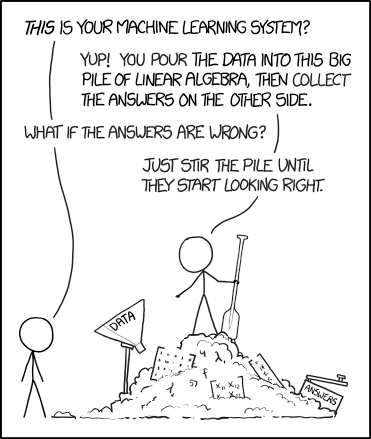
\includegraphics[height=0.55\textheight]{images/1838_machine_learning.png}
\end{column}
\begin{column}{0.50\textwidth}
\vspace{5mm}
You already know \textbf{what embeddings are} (L06a).

\vspace{3mm}
Now: how do practitioners actually \highlight{USE} them today?

\vspace{3mm}
\begin{compactlist}
\item Sentence-level embeddings
\item Semantic search and RAG
\item Vector databases
\end{compactlist}
\end{column}
\end{columns}
\bottomnote{XKCD \#1838 by Randall Munroe (CC BY-NC 2.5)}
\end{frame}

% ---------- Slide 3: TikZ Comic C1 ----------
\begin{frame}{The Problem: So Many Documents!}
\begin{center}
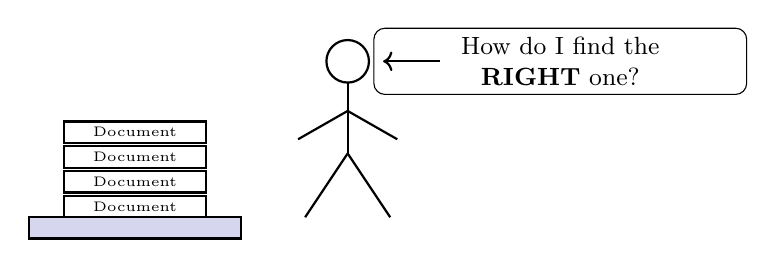
\begin{tikzpicture}[scale=0.9]
% Desk
\draw[thick, fill=mllavender4] (0,0) rectangle (3,0.3);
% Document stack
\foreach \i in {0,0.35,0.7,1.05} {
  \draw[thick, fill=white] (0.5,0.3+\i) rectangle (2.5,0.6+\i);
  \node[font=\tiny] at (1.5,0.45+\i) {Document};
}
% Stick figure
\draw[thick] (4.5,2.5) circle (0.3);
\draw[thick] (4.5,2.2) -- (4.5,1.2);
\draw[thick] (4.5,1.8) -- (3.8,1.4);
\draw[thick] (4.5,1.8) -- (5.2,1.4);
\draw[thick] (4.5,1.2) -- (3.9,0.3);
\draw[thick] (4.5,1.2) -- (5.1,0.3);
% Speech bubble
\node[draw, rounded corners, fill=white, font=\small,
      text width=4.5cm, align=center] at (7.5,2.5)
  {How do I find the \textbf{RIGHT} one?};
\draw[->, thick] (5.8,2.5) -- (5.0,2.5);
\end{tikzpicture}
\end{center}
\vspace{2mm}
Modern embeddings solve this: they let you \highlight{search by meaning}, not keywords.
\bottomnote{Keyword search fails when the user says ``revenue'' but the document says ``income''.}
\end{frame}

% ---------- Slide 4: From Words to Sentences ----------
\begin{frame}{From Words to Sentences}
\begin{columns}[T]
\begin{column}{0.47\textwidth}
\textcolor{mlred}{\textbf{Word Embeddings (L06a)}}
\begin{compactlist}
\item One vector per \textbf{word}
\item ``bank'' always the same vector
\item Word2Vec, GloVe
\end{compactlist}
\end{column}
\begin{column}{0.47\textwidth}
\textcolor{mlgreen}{\textbf{Sentence Embeddings (Today)}}
\begin{compactlist}
\item One vector per \textbf{sentence}
\item Captures full meaning
\item sentence-transformers
\end{compactlist}
\end{column}
\end{columns}
\vspace{4mm}
\begin{block}{Key Insight}
Modern applications embed \highlight{sentences}, not individual words.
\end{block}
\bottomnote{sentence-transformers is the most popular library: 100M+ downloads on Hugging Face.}
\end{frame}

% ---------- Slide 5: The Key Players ----------
\begin{frame}{The Key Players in 2025}
\begin{compactlist}
\item \textbf{Open source:} sentence-transformers\\
      Models: \texttt{all-MiniLM-L6-v2}, \texttt{all-mpnet-base-v2}
\item \textbf{API-based:} OpenAI (\texttt{text-embedding-3-small}), Cohere (\texttt{embed-v3}), Voyage AI
\item \textbf{Leaderboard:} MTEB on Hugging Face ranks hundreds of models by task
\end{compactlist}
\bottomnote{Tip: start with all-MiniLM-L6-v2 (free, fast, good). Upgrade to API models if you need top accuracy.}
\end{frame}

% ---------- Slide 6: TikZ Diagram D1 ----------
\begin{frame}[fragile]{Sentence vs.\ Word Embedding}
\begin{center}
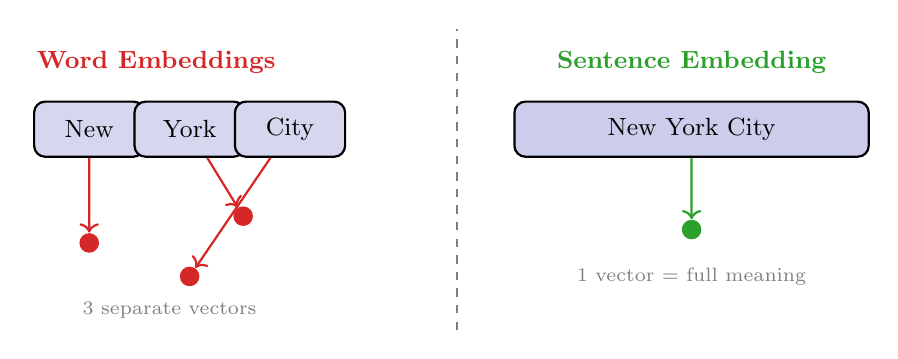
\begin{tikzpicture}[scale=0.85,
    wordbox/.style={draw, thick, rounded corners, fill=mllavender4,
                    minimum height=0.7cm, minimum width=1.4cm, font=\small},
    sentbox/.style={draw, thick, rounded corners, fill=mllavender3,
                    minimum height=0.7cm, minimum width=4.5cm, font=\small},
    dot/.style={circle, fill=#1, inner sep=2.5pt}]
% Left: word embeddings
\node[font=\bfseries\small, text=mlred] at (-4.5,3) {Word Embeddings};
\node[wordbox] (w1) at (-5.5,2) {New};
\node[wordbox] (w2) at (-4.0,2) {York};
\node[wordbox] (w3) at (-2.5,2) {City};
\node[dot=mlred] (d1) at (-5.5,0.3) {};
\node[dot=mlred] (d2) at (-3.2,0.7) {};
\node[dot=mlred] (d3) at (-4.0,-0.2) {};
\draw[->, thick, mlred] (w1) -- (d1);
\draw[->, thick, mlred] (w2) -- (d2);
\draw[->, thick, mlred] (w3) -- (d3);
\node[font=\scriptsize, text=mlgray] at (-4.3,-0.7) {3 separate vectors};
% Right: sentence embedding
\node[font=\bfseries\small, text=mlgreen] at (3.5,3) {Sentence Embedding};
\node[sentbox] (s1) at (3.5,2) {New York City};
\node[dot=mlgreen] (d4) at (3.5,0.5) {};
\draw[->, thick, mlgreen] (s1) -- (d4);
\node[font=\scriptsize, text=mlgray] at (3.5,-0.2) {1 vector = full meaning};
% Divider
\draw[dashed, thick, mlgray] (0,-1) -- (0,3.5);
\end{tikzpicture}
\end{center}
\vspace{1mm}
Sentence embeddings understand that ``New York City'' is \textbf{one concept}, not three words.
\bottomnote{Technical detail: sentence-transformers use mean pooling over token embeddings from a transformer model.}
\end{frame}

% ---------- Slide 7: Similarity Heatmap (reused chart) ----------
\begin{frame}{Semantic Search = Cosine Similarity}
\begin{columns}[T]
\begin{column}{0.55\textwidth}

\includegraphics[width=\textwidth]{02_similarity_heatmap/chart.pdf}
\end{column}
\begin{column}{0.40\textwidth}
\vspace{3mm}
\begin{compactlist}
\item This is the \textbf{core operation} behind semantic search
\item Compute cosine similarity between query and document embeddings
\item Darkest cell = most relevant result
\end{compactlist}
\end{column}
\end{columns}
\bottomnote{Cosine similarity ranges from $-1$ (opposite) to $+1$ (identical). In practice, scores above 0.7 are strong matches.}
\end{frame}

% ---------- Slide 8: RAG Pipeline (new chart) ----------
\begin{frame}{RAG: The \#1 Pattern for Embeddings + LLMs}
\begin{center}

\includegraphics[width=0.65\textwidth]{14_rag_pipeline_flow/chart.pdf}
\end{center}
\vspace{1mm}
\begin{compactlist}
\item \textbf{RAG} = Retrieval-Augmented Generation
\item Embed your documents once, retrieve on every question
\item No retraining needed --- works with any LLM
\end{compactlist}
\bottomnote{RAG lets an LLM answer questions about YOUR documents without retraining. Used at JPMorgan, Bloomberg, every major bank.}
\end{frame}

% ---------- Slide 9: TikZ Comic C2 ----------
\begin{frame}{The Smart Librarian: How RAG Works}
\begin{center}
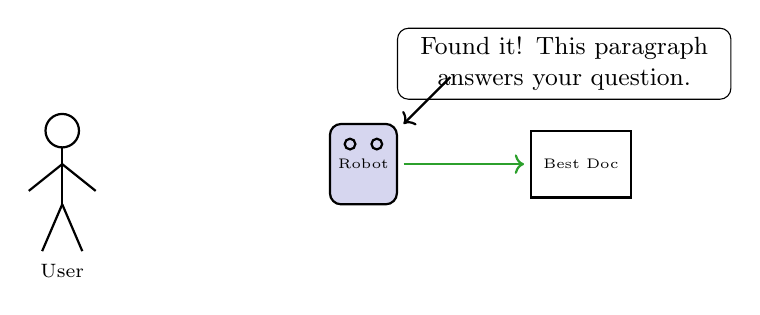
\begin{tikzpicture}[scale=0.85]
% Librarian stick figure
\draw[thick] (-3,2.5) circle (0.25);
\draw[thick] (-3,2.25) -- (-3,1.4);
\draw[thick] (-3,2.0) -- (-3.5,1.6);
\draw[thick] (-3,2.0) -- (-2.5,1.6);
\draw[thick] (-3,1.4) -- (-3.3,0.7);
\draw[thick] (-3,1.4) -- (-2.7,0.7);
\node[font=\scriptsize] at (-3,0.4) {User};
% Robot
\draw[thick, fill=mllavender4, rounded corners] (1,1.4) rectangle (2,2.6);
\node[font=\tiny] at (1.5,2.0) {Robot};
\draw[thick] (1.3,2.3) circle (0.08);
\draw[thick] (1.7,2.3) circle (0.08);
% Document
\draw[thick, fill=white] (4,1.5) rectangle (5.5,2.5);
\node[font=\tiny] at (4.75,2.0) {Best Doc};
% Arrow robot to doc
\draw[->, thick, mlgreen] (2.1,2.0) -- (3.9,2.0);
% Speech bubble
\node[draw, rounded corners, fill=white, font=\small,
      text width=4cm, align=center] at (4.5,3.5)
  {Found it! This paragraph answers your question.};
\draw[->, thick] (2.8,3.3) -- (2.1,2.6);
\end{tikzpicture}
\end{center}
\vspace{1mm}
\begin{enumerate}\setlength{\itemsep}{1pt}
\small
\item Embed documents once, store vectors in a database (FAISS, ChromaDB, Pinecone)
\item When a question arrives, embed it and find the nearest documents
\item Feed those documents to an LLM for a precise answer
\end{enumerate}
\bottomnote{Vector databases: FAISS (Meta, free), ChromaDB (open source), Pinecone (cloud). All work with sentence-transformers.}
\end{frame}

% ---------- Slide 10: Python Code ----------
\begin{frame}{Try It Yourself --- Six Lines to Semantic Search}
\begin{center}
\footnotesize
\begin{tabular}{l}
\texttt{from sentence\_transformers import SentenceTransformer} \\
\texttt{model = SentenceTransformer("all-MiniLM-L6-v2")} \\
\\
\texttt{docs = ["Annual revenue rose 12\%",} \\
\texttt{~~~~~~~~"Q3 losses exceeded forecast"]} \\
\texttt{query = "How did the company perform financially?"} \\
\\
\texttt{doc\_embeddings = model.encode(docs)} \\
\texttt{query\_embedding = model.encode(query)} \\
\texttt{\# Use cosine similarity to find the best match!} \\
\end{tabular}
\end{center}
\vspace{2mm}
That's it --- \highlight{six lines} to build a semantic search engine.
\bottomnote{pip install sentence-transformers. Free, runs locally, no API key needed. Hugging Face Hub has 5000+ embedding models.}
\end{frame}

% ---------- Slide 11: XKCD Closing ----------
\begin{frame}{What Could Possibly Go Wrong?}
\begin{center}
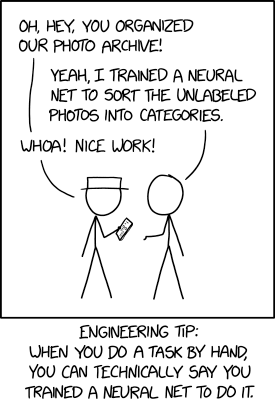
\includegraphics[height=0.55\textheight]{images/2173_trained_a_neural_net.png}
\end{center}
\bottomnote{XKCD \#2173 by Randall Munroe (CC BY-NC 2.5). Next: try the RAG notebook with real financial filings!}
\end{frame}

\end{document}
